It has been known for a long time that gravitational energy is insufficient to completely power the sun for its lifetime; however, in recent decades, it has become apparent that there are other contexts in which gravitation is the \textbf{sole adequate engine} for a number of different phenomena. This includes AGN and quasars, TDEs, and a number of other observed systems featuring compact objects.
\par
In a general sense, we might consider a system containing a compact object of mass $M$ and radius $R$. If a mass $m$ falls from $\infty$ into the surface of the compact object, it will gain
\[
K = \frac{GMm}{R}
\]
in kinetic energy.
\vspace{0.25cm}
\begin{itemize}
    \item For \textbf{stellar objects}, the kinetic energy per unit mass extracted from this process is
    \[
    \epsilon = 2 \times 10^{15}\left(\frac{M}{M_\odot}\right)\left(\frac{R}{R_\odot}\right)^{-1} \;{\rm erg\;s^{-1}}.
    \]
    \item For \textbf{compact objects}, where $GM/R \sim c^2$, one finds instead that
    \[
    \epsilon \approx 9\times 10^{20}\;{\rm erg\;s^{-1}}.
    \]
\end{itemize}
\vspace{0.25cm}
For reference, a nuclear reaction with efficiency $\eta$ would yield
\[
\epsilon \approx \eta c^2, \;\text{for typical $\eta \sim 10^{-3}$,}\; \epsilon \approx 10^{18}\;{\rm erg\; s^{-1}}.
\]
Thus, we see that while \textbf{gravitational energy is subdominant for stellar objects}, it can be \textbf{highly energetic for compact objects}.
\par

\begin{bigidea}
    The study of accretion is the study of two effects:
\begin{enumerate}
    \item The \textbf{flow of material to the surface of the accretor}, which is a largely well understood problem, and
    \item The \textbf{radiation of energy / distribution of angular momentum}, which remains a very active field of research in astrophysics to this day.
\end{enumerate}
\end{bigidea}

\section{The Eddington Limit}

In this section, we introduce the \textbf{Eddington accretion limit}, which is an effective metric for the limitation of "normal" accretion.
\par
Consider an accretion scenario in which \textbf{fully ionized Hydrogen} accretes onto a central body. If that central body has a bolometric luminosity $L_{\rm bol}$, then the incident photons will exert a \textbf{radiation pressure} on the in-falling material. The energy transport per unit area at distance $r$ from the surface is
\[
|{\bf S}| = \frac{L_{\rm bol}}{4\pi r^2} \implies P_{\rm rad} = \frac{L_{\rm bol}}{4\pi r^2 c}.
\]
The dominant interaction mechanism with be \textbf{Thompson scattering off free electrons}, and so the Thompson cross section determines the relevant force on the particles:
\[
F = \frac{L_{\rm bol}\sigma_T}{4\pi r^2 c}.
\]
\rmk{There are actually two statements here that get swept under the rug. First off, we assume Thompson scattering is dominant over other forms of interaction. This is fine \textit{if} we don't have magnetic fields or very high temperature gas. As long as we are below $\sim 100\;{\rm keV},$ we're still in the non-relativistic regime of Thompson and don't have to treat Compton. We also recognize that $\sigma_{\rm thompson} \sim r_0^2 \sim m^{-2}$, so the electrons are the dominant source of scatter, not the protons. Because they are tightly coupled, both will effectively get dragged along.}
\par
Now, the gravitational force per electron-proton pair is
\[
F_{\rm grav} = - \frac{GM(m_p+m_e)}{r^2} \approx - \frac{GMm_p}{r^2},
\]
so
\[
F \le 0 \implies \frac{GMm_p}{r^2} \ge \frac{L_{\rm bol} \sigma_T}{4\pi r^2 c} \implies L_{\rm bol} = 4\pi G M m_p c / \sigma_T.
\]
This leads us to the formal definition of the \textbf{Eddington Luminosity}:
\vspace{0.5cm}
\begin{definition}[Eddington Luminosity]
The \textbf{Eddington Luminosity} is defined to be
\begin{equation}
    \label{eq:eddington_luminosity}
    \boxed{
    L_{\rm Edd} = \frac{4\pi GMm_p c}{\sigma_T} = 1.3 \times 10^{38} \; \left(\frac{M}{M_\odot}\right) \;\rm{ergs\;s^{-1}}.
    }
\end{equation}
It is the \textbf{maximum luminosity at which accretion can occur}.
\end{definition}


\subsection{Super-Eddington Sources}
The derivation of the Eddington luminosity implicitly assumes several caveats:
\vspace{0.25cm}
\begin{enumerate}
    \item \textbf{Interaction mechanism:} We assume that the dominant coupling between photons and matter is \emph{Thomson scattering} off free electrons. This is valid as long as the characteristic photon energies are $\lesssim 100 \,{\rm keV}$, so that Klein--Nishina (Compton) corrections are negligible, and no strong magnetic fields introduce cyclotron or resonant scattering processes.
    \item \textbf{Scatterers:} Because $\sigma_T \propto m^{-2}$, electrons dominate the scattering cross section compared to protons. Electrons and protons are coupled via Coulomb forces, so the radiation effectively drags along the entire electron--proton plasma.
    \item \textbf{Opacity:} We treat the opacity as a pure scattering opacity given by $\kappa = \sigma_T/m_p$. In realistic astrophysical systems, bound-free absorption, free-free opacity, or dust scattering may be important and can modify the effective Eddington limit.
    \item \textbf{Geometry and symmetry:} The calculation assumes spherical symmetry and isotropic radiation. In accretion disks, anisotropic emission and beaming effects can allow accretion to exceed the nominal Eddington luminosity locally.
    \item \textbf{Steady-state assumption:} The Eddington limit describes a balance between radiation pressure and gravity in an ideal steady-state system. Transient or time-dependent accretion flows may temporarily surpass $L_{\rm Edd}$.
\end{enumerate}
\vspace{0.25cm}
Thus, while $L_{\rm Edd}$ provides a robust benchmark for the ``normal'' luminosity limit of accreting systems, real astrophysical environments can deviate from this simple picture. There are many examples of such systems:
\vspace{0.25cm}
\begin{itemize}
    \item \textbf{Ultraluminous X-ray sources (ULXs):} Compact objects in external galaxies with apparent luminosities $\gtrsim 10^{39}\,\mathrm{erg\,s^{-1}}$, above the Eddington limit for a stellar-mass black hole. These are thought to involve either beaming effects or accretion onto neutron stars with strong magnetic fields.
    \item \textbf{Tidal disruption events (TDEs):} When a star is torn apart by a supermassive black hole, the fallback of stellar debris can briefly power emission well above the Eddington luminosity.
    \item \textbf{Supermassive black hole growth (quasars):} Some quasars, especially in the early universe, show evidence for sustained super-Eddington accretion, which may explain how black holes grew rapidly to billions of solar masses within a few hundred million years.
\end{itemize}
\vspace{0.25cm}
In short, while the Eddington luminosity provides a useful benchmark, nature finds several ways to circumvent it, making super-Eddington accretion a key ingredient in high-energy astrophysics.

\section{Characterizing Accretion Emission}

\subsection{The Accretion Luminosity}
The fact that there is a natural scale for viable accretion powered luminosity, it becomes worth asking the question: \textbf{how much luminosity do we get from accretion?} In general, this is a complex question and not easily constrained; however, we might make a broad characterization by defining the \textbf{accretion luminosity}, which is the \textit{total released energy assuming perfect conversion}:
\begin{equation}
    \label{eq:accretion_luminosity}
    \boxed{
    L_{\rm acc} = \frac{GM\dot{M}}{R} = \begin{cases}
        1.3 \times 10^{33} \;\dot{M}_{16} \left(\frac{M}{M_\odot}\right) \left(\frac{10^9\;{\rm cm}}{R}\right)\;{\rm ergs\;s^{-1}},&\text{W.D.}\\
        1.3 \times 10^{36}  \;\dot{M}_{16} \left(\frac{M}{M_\odot}\right) \left(\frac{10^6\;{\rm cm}}{R}\right)\;{\rm ergs\;s^{-1}},&\text{N.S.}
    \end{cases}
    }
\end{equation}
where $\dot{M} = 10^{16}\;\dot{M}_{16} \;{\rm g\;s^{-1}}.$ \rmk{For accretion onto binary systems, $\dot{M}_{16}\sim 1$ for most systems, justifying its introduction.} 
\begin{remark}
    We \textbf{formally} acknowledge that $L_{\rm acc} \neq L_{\rm Obs}$ in most relevant scenarios. $L_{\rm acc}$ is not really the \textbf{observed luminosity}, but instead the upper bound on the luminosity. 
\end{remark}
\par
The above equation relies on our ability to specify a relevant $R$; however, we might actually have energy released at lower radii or inefficient energy release. We therefore introduce a \textbf{alternative definition}
\begin{equation}
    L_{\rm acc} = \eta c^2 \dot{M},
\end{equation}
where $\eta$ is the \textbf{accretion efficiency}. 
\begin{remark}
    $\eta$ is a \textbf{tricky parameter} because the theorist will draw a distinction between $\eta = L_{\rm acc}/(\eta \dot{M})$ while the observer will say that $\eta = L_{\rm Obs}/(\eta \dot{M})$. We may also apply this definition for \textbf{non-compact objects with definite radius}: $\eta$ swallows up the weird dependencies on $G$ and $R$.
\end{remark}
Based on this, we can let $L_{\rm acc} = L_{\rm Edd}$ and therefore derived the very important \textbf{Eddington Accretion Rate (EAR)}
\begin{equation}
\boxed{
    \dot{M}_{\rm Edd} = \frac{L_{\rm Edd}}{\eta c^2} = \frac{4\pi G M m_p}{\sigma_T \eta c}}
\end{equation}
The relevant scaling goes as
\[
 \dot{M}_{\rm Edd} = \eta^{-1}\; 1.4 \times 10^{17}\; \left(\frac{M}{M_\odot}\right)\;{\rm g\; s^{-1}} = \eta^{-1}\;2.2 \times 10^{-9} \left(\frac{M}{M_\odot}\right)\; {\rm M_\odot\;yr^{-1}}.
\]


\subsection{The Emitted Spectrum}

An important question in accretion physics is: \textbf{what spectrum of radiation is produced by the accretion flow?}  The answer depends on how efficiently the liberated gravitational energy thermalizes and how photons interact with the surrounding medium.  Several characteristic temperatures are useful for bounding the expected emission. The first of which is the estimated, intrinsic temperature of the emitted photons:
\vspace{0.5cm}
\begin{definition}[Radiation Temperature]
\label{def:rad_temperature}
The \textbf{radiation temperature} $T_{\rm rad}$ is the effective temperature of the emergent photons,
\begin{equation}
    \label{eq:rad_temp}
    T_{\rm rad} = \frac{h\left<\nu\right>}{k_b} = 1.16\times 10^{7} \left(\frac{h\bar{\nu}}{1\;{\rm keV}}\right)\;{\rm K}.
\end{equation}
\end{definition}
\vspace{0.5cm}

Now, depending on the nature of the source, $T_{\rm rad}$ may range considerably. There are a number of other proxies which are used and which provide useful order-of-magnitude bounds for $T_{\rm rad}$.
\vspace{0.25cm}
\begin{definition}[Thermal Temperature]
\label{def:thermal_temperature}
The \textbf{thermal temperature} $T_{\rm thermal}$ is the temperature obtained if the full gravitational potential energy released by accretion were converted into thermal energy of the gas. Formally, for a monatomic gas, 
\begin{equation}
    \label{eq:thermal_temperature}
    T_{\rm thermal} = \frac{GMm_p}{3k_bR}= \frac{2U_{\rm grav, proton}}{k_b}. 
\end{equation}
It provides an \emph{upper bound} on heating. In principle, if accretion is highly efficient and optically thin, we expect emission to have a characteristic temperature similar to $T_{\rm thermal}$.
\end{definition}
\vspace{0.25cm}
\begin{definition}[Virial Temperature]
\label{def:virial_temperature}
The \textbf{virial temperature} $T_{\rm virial}$ characterizes gas in virial equilibrium, where the thermal energy is about half of the gravitational potential energy. 
Thus, $T_{\rm virial} \simeq \tfrac{1}{2}T_{\rm thermal}$, making it a more realistic estimate for the gas near the accretor.
\end{definition}
\vspace{0.25cm}
\begin{definition}[Brightness Temperature]
\label{def:brightness_temperature}
The \textbf{brightness temperature} $T_b$ is the blackbody temperature a source would need to radiate the observed flux. 
\begin{equation}
    \label{eq:brightness_temperature}
    T_b = \left(\frac{L_{\rm acc}}{4\pi R^2 \sigma_{\rm sb}}\right)^{1/4}.
\end{equation}
It serves as the observable counterpart to $T_{\rm rad}$ in the optically thick case and is generally a a good lower bound on $T_{\rm rad}$.
\end{definition}
\vspace{0.5cm}

\begin{bigidea}
    The emitted spectrum of an accretion flow is bounded by these characteristic scales:  
    \[
    T_{\rm virial} \;\;\lesssim\;\; T_{\rm rad},\,T_b \;\;\lesssim\;\; T_{\rm thermal}.
    \]  
    \textbf{Takeaway:} The precise emission depends on opacity and optical depth, but these temperatures provide natural limits on what can be observed.
\end{bigidea}

\section{Accreting Systems and Their Properties}
\begin{figure}[ht!]
    \centering
    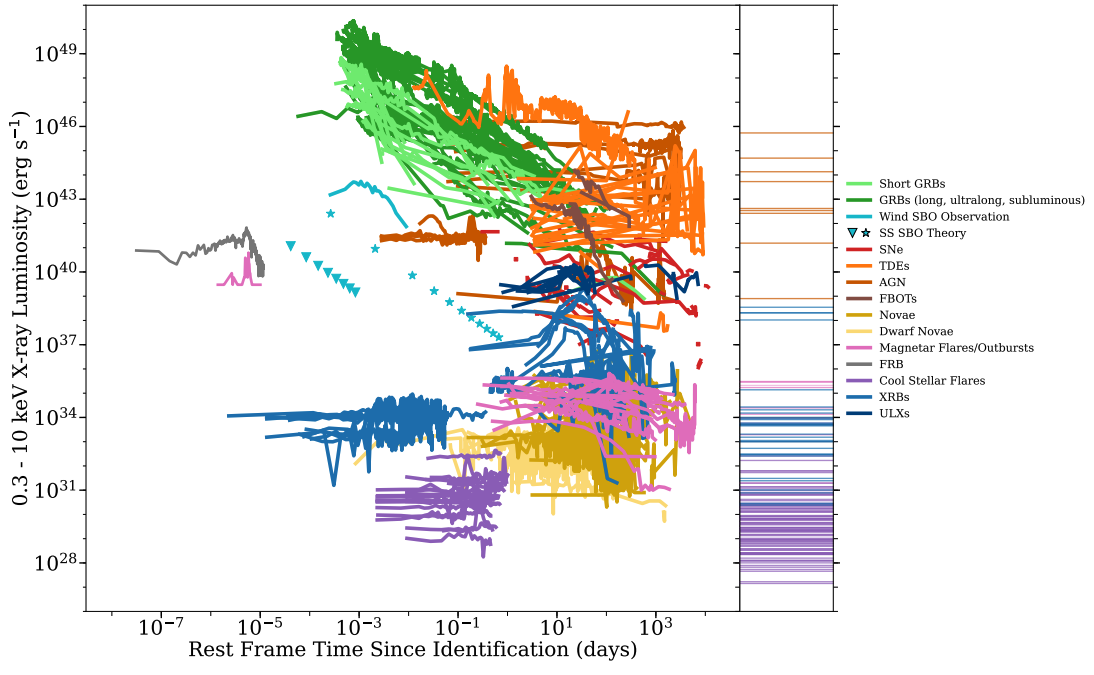
\includegraphics[width=\linewidth]{Pictures/figures/xray_sources.png}
    \caption{X-ray phase space of transients and variable phenomena, including gamma-ray burst (GRB) afterglows, supernovae (SNe), supernova shock breakouts (SBOs), tidal disruption events (TDEs) and active galactic nuclei (AGN), fast blue optical transients (FBOTs), cataclysmic variables, magnetar flares/outbursts and fast radio bursts, cool stellar flares, X-ray binary outbursts, and ultraluminous X-ray sources. Main Panel: X-ray luminosity evolution with rest-frame time since identification. Theoretical SBO peak Lx-duration points are shown with different symbols corresponding to the model’s input parameters; see Section 2.2 for details. Right Side Panel: To offer a sense of their persistent behavior, the quiescent/pre-flare luminosities of the included variable classes (AGN, magnetar flares/outbursts, cool stellar flares, X-ray binaries, and ultraluminous X-ray sources) are shown as horizontal bars. Taken from Polzin+ 2023}
    \label{fig:xray_sources}
\end{figure}

Before completing this section introducing accretion, it is worth tabulating classic scenarios where accretion is relevant, whether or not they are sub or super-Eddington, what their typical accretion rates and efficiencies are, etc. In doing so, the resulting tables will provide a helpful reference when considering many of the methods / mechanisms below. One of the major takeaways should be the relevant eddington accretion rates for the various types of compact objects. In most scenarios (see Table~\ref{tab:compact-objects}), sources need very little accretion to reach their Eddington limit. Notably, the mass dependence of black holes means that for stellar mass black holes, we need only $\sim 10^{-8} \;{\rm M_\odot \; yr^{-1}}$ to reach $L_{\rm Edd}$, but for a supermassive black hole at (say) $10^{8} {\rm M_\odot}$ or larger, we $\sim 1\;{\rm M_\odot\; yr^{-1}}$.
\begin{table}[h]
    \small
    \centering
    {
    \renewcommand{\arraystretch}{2}
    \begin{tabular}{p{2cm}|p{3cm}p{3cm}p{5cm}}
        \hline
        \textbf{Object Type} & \textbf{White Dwarfs} & \textbf{Neutron Stars} & \textbf{Black Holes} \\
        \hline
        Mass & $\sim 1\,M_\odot$ 
                  & $\sim 1.4\,M_\odot$ 
                  & $\sim 1\!-\!10^{8}\,M_\odot$ \\
                \hline
        Radius & $\sim 5000\,{\rm km} \approx R_\oplus$ 
                    & $\sim 10\,{\rm km}$ 
                    & Not well defined \\
                \hline
        $L_{\rm Edd}$ & $1.3 \times 10^{38}\,{\rm erg\,s^{-1}}$ 
                      & $1.3 \times 10^{38}\,{\rm erg\,s^{-1}}$ 
                      & $1.38 \times 10^{38}\,(M/M_\odot)\,{\rm erg\,s^{-1}}$ \\
                \hline
        $\dot{M}_{\rm Edd}$ & $8 \times 10^{-6}\,M_\odot\,{\rm yr^{-1}}$ 
                            & $1.6 \times 10^{-8}\,M_\odot\,{\rm yr^{-1}}$ 
                            & $2 \times 10^{-9}\,(M/M_\odot)\,\eta^{-1}\,M_\odot\,{\rm yr^{-1}}$ \\
                \hline
        $\eta$ (nominal / modeled) & $\sim 3 \times 10^{-4}$ 
                                   & $\sim 0.15$ 
                                   & $\sim 0.1$ (model-dependent) \\
        \hline
    \end{tabular}
    }
    \caption{Representative properties of compact objects and their Eddington limits.}
    \label{tab:compact-objects}
\end{table}

\begin{table}[h]
    \small
\centering
\renewcommand{\arraystretch}{1.2}
\begin{tabular}{lcccc}
\hline
\textbf{Object} & \textbf{$L_{X,\rm obs}$} & \textbf{Lower limit on $M$} & \textbf{$\dot{M}$ if $L_{\rm obs}=L_{\rm acc}$} & \textbf{Eddington regime} \\
                & (erg s$^{-1}$) & ($M_\odot$) & ($M_\odot$ yr$^{-1}$) &  \\
\hline
Novae           & $\sim 10^{33}$ & $> 10^{-5}$ & $6 \times 10^{-11}$ & Sub-Edd.\\
WD              &                &             &                      &             \\
\hline
XRBs            & $10^{34} - 10^{38}$ & $> 10^{-4} - 1$ & $10^{-12} - 10^{-8}$ & Sub-Edd.\\
BH, NS          &                     &                 &                      &             \\
\hline
LERGBs / SGRBs  & up to $10^{49}$ & $> 10^{11}$ & $\sim 10^{3}$ & Super-Edd. \\
BH, NS          &                 &             &               &             \\
\hline
TDEs            & $10^{38} - 10^{49}$ & $> 1 - 10^{9}$ & $10^{-8} - 1$ & SMBH\\
SMBH            &                     &                 &               &        \\
\hline
AGNs            & $10^{40} - 10^{49}$ & $> 10^{2} - 10^{9}$ & $10^{-6} - 10^{-7}$ & SMBH\\
SMBH            &                     &                     &                      &         \\
\hline
SNe             & $\sim 10^{40}$ & $> 10^{2}$ & $10^{-6}$ & Super-Edd. \\
BH, NS          &                 &            &           &                           \\
\hline
ULXs            & $\sim 10^{40}$ & $> 10^{2}$ & $10^{-6}$ & IMBH or Super-Edd. \\
BH, NS          &                 &            &           &                           \\
\hline
\end{tabular}
\caption{Representative accreting systems, observed luminosities, implied minimum masses, and accretion rates assuming $L_{\rm obs}=L_{\rm acc}$. The last column indicates whether the system is consistent with sub- or super-Eddington accretion.}
\label{tab:accretion-systems}
\end{table}

\subsection{Novae}
Cataclysmic variables can be divided into three main classes: \emph{classical novae}, 
\emph{recurrent novae}, and \emph{dwarf novae}. In classical novae, a white dwarf accretes material 
from a main-sequence companion star until the accumulated hydrogen undergoes runaway nuclear fusion, 
producing a dramatic outburst. Recurrent novae follow the same mechanism but exhibit regular, 
periodic eruptions on much shorter timescales. Dwarf novae are fainter systems in which instabilities 
in the accretion disk drive more frequent, but less luminous, eruptions.  
Typical X-ray luminosities fall in the range $10^{31}$--$10^{34}\,{\rm erg\,s^{-1}}$, implying 
a lower limit on the white dwarf accretor mass of about $10^{-5}\,M_\odot$. 
Accretion rates are correspondingly low, on the order of 
$\dot{M} \sim 10^{-11}\,M_\odot\,{\rm yr^{-1}}$, comfortably consistent with sub-Eddington accretion.

\subsection{X-ray Binaries (XRBs)}
X-ray binaries are systems in which a neutron star or black hole accretes from a stellar companion. 
They are typically categorized into low-, intermediate-, and high-mass XRBs depending on the nature 
of the donor star. Unlike novae, the compactness of neutron stars and black holes allows for much more 
efficient conversion of gravitational potential energy into radiation, making these systems far more 
luminous. Observed X-ray luminosities span a wide range, from $10^{34}$ up to $10^{38}\,{\rm erg\,s^{-1}}$. 
The presence of such luminosities requires an accretor mass of at least $\sim 1\,M_\odot$, 
consistent with the expected masses of neutron stars and stellar-mass black holes. 
The implied mass accretion rates are modest, in the range 
$\dot{M} \sim 10^{-12}$--$10^{-8}\,M_\odot\,{\rm yr^{-1}}$, which again fall within the 
sub-Eddington regime for these compact objects.

\subsection{Gamma-Ray Bursts (GRBs)}
Gamma-ray bursts (GRBs) are among the most luminous transients in the universe, 
associated with the collapse of massive stars (long GRBs) or the merger of compact objects such as 
neutron stars (short GRBs). These events channel enormous amounts of energy into highly relativistic jets, 
producing brief but intense bursts of gamma rays. Observed luminosities can reach up to 
$10^{49}\,{\rm erg\,s^{-1}}$, far exceeding the Eddington limit for stellar-mass objects. 
To sustain such emission, accretor masses of order $10^{11}\,M_\odot$ would be required under the 
Eddington argument, which is unphysical. Instead, the implied accretion rates are extreme, 
$\dot{M} \sim 10^{3}\,M_\odot\,{\rm yr^{-1}}$, demonstrating that GRBs operate in a 
super-Eddington regime where relativistic jet physics, not steady-state accretion, dominates the 
energy output.

\subsection{Tidal Disruption Events (TDEs)}
Tidal disruption events occur when a star passes close enough to a supermassive black hole to be torn 
apart by tidal forces. Roughly half the stellar debris becomes unbound, while the remainder accretes 
rapidly onto the black hole, producing a luminous X-ray/UV flare. Observed luminosities span 
$10^{38}$ to $10^{49}\,{\rm erg\,s^{-1}}$, corresponding to black hole masses in the range 
$10^{1}$ to $10^{9}\,M_\odot$. The implied accretion rates range from 
$\dot{M} \sim 10^{-8}$ up to $1\,M_\odot\,{\rm yr^{-1}}$, consistent with supermassive black holes 
and often approaching or exceeding the Eddington limit. These events highlight how black holes can 
transiently accrete at highly super-Eddington rates following stellar disruption.

\subsection{Active Galactic Nuclei (AGN)}
Active galactic nuclei represent sustained accretion onto supermassive black holes at the centers of 
galaxies. Accretion disks in AGN convert gravitational binding energy into radiation with high 
efficiency, powering emission across the electromagnetic spectrum. Typical luminosities range from 
$10^{40}$ to $10^{49}\,{\rm erg\,s^{-1}}$, requiring black hole masses of $10^{2}$ to $10^{9}\,M_\odot$. 
Inferred mass accretion rates fall between $\dot{M} \sim 10^{-7}$ and $10^{-6}\,M_\odot\,{\rm yr^{-1}}$, 
sufficient to sustain steady growth of supermassive black holes over cosmic timescales. These values 
remain broadly consistent with Eddington-limited accretion, though some AGN show evidence of mildly 
super-Eddington behavior.

\subsection{Ultra-Luminous X-ray Sources (ULXs)}
Ultra-luminous X-ray sources are extragalactic, off-nuclear point sources with X-ray luminosities that 
exceed the Eddington limit for a typical stellar-mass black hole. Observed values cluster around 
$L_X \sim 10^{40}\,{\rm erg\,s^{-1}}$, which would require accretors more massive than 
$100\,M_\odot$ if powered purely by sub-Eddington accretion. The implied mass accretion rates are 
$\dot{M} \sim 10^{-6}\,M_\odot\,{\rm yr^{-1}}$. This has led to two interpretations: either ULXs host 
intermediate-mass black holes accreting near the Eddington limit, or they are stellar-mass black holes 
and neutron stars accreting at genuinely super-Eddington rates. Observations of pulsating ULXs confirm 
that, at least in some cases, neutron stars can sustain super-Eddington accretion with the aid of strong 
magnetic fields and beaming.
